\documentclass{anstrans}
%%%%%%%%%%%%%%%%%%%%%%%%%%%%%%%%%%%
\title{Assessing Material Inventory Uncertainties in Integrated Fuel Cycle Simulations}
\author{Baptiste Mouginot, Kathryn Mummah, Paul P.H.  Wilson}

\institute{
University of Wisconsin-Madison, Madison, WI
}

\email{mouginot@wisc.edu \and mummah@wisc.edu \and paul.wilson@wisc.edu}

% Optional disclaimer: remove this command to hide
% \disclaimer{Notice: this manuscript is a work of fiction.  Any resemblance to
% actual articles, living or dead, is purely coincidental.}

%%%% packages and definitions (optional)
\usepackage{graphicx} % allows inclusion of graphics
\usepackage{booktabs} % nice rules (thick lines) for tables
\usepackage{microtype} % improves typography for PDF
\usepackage{float}

\newcommand{\SN}{S$_N$}
\renewcommand{\vec}[1]{\bm{#1}} %vector is bold italic
\newcommand{\vd}{\bm{\cdot}} % slightly bold vector dot
\newcommand{\grad}{\vec{\nabla}} % gradient
\newcommand{\ud}{\mathop{}\!\mathrm{d}} % upright derivative symbol
\newcommand{\ie}{\emph{i.e.\ }}

\usepackage[acronym]{glossaries}
\newacronym{UOX}{UOX}{uranium oxide fuel}
\newacronym{MOX}{MOX}{mixed oxide fuel}
\newacronym{LWR}{LWR}{light water reactor}
\newacronym{SFR}{SFR}{fast breeder reactor}
\newacronym{OFAT}{OFAT}{one-factor-at-a-time}

\begin{document}
%%%%%%%%%%%%%%%%%%%%%%%%%%%%%%%%%%%%%%%%%%%%%%%%%%%%%%%%%%%%%%%%%%%%%%%%%%%%%%%%
\section{Introduction}

Fuel cycle simulations, as with any simulation process, do not produce results
without uncertainties.  Those uncertainties have two main sources: modeling
uncertainty due to the simplifications and approximations built in to the
simulator itself, and data uncertainty from the quantities provided by the user.
This work focuses on a subset the data uncertainty related to the user input
that defines the performance of the simulated facilities.

Such simulation uncertainties could be important in the context of treaty
verification.  Some scenarios require estimating historical fissile material
production based on records of facility operation and material transfer.  If the
measurements of facility operation and material transfer are subject to
uncertainty, the total production quantities will then also be uncertain.  Any
uncertainty in fissile production quantities poses a material accounting
challenge, possibly creating an opportunity for undetected diversion.

This study seeks to understand which characteristics of facility operation have
the most impact on the uncertainty of fissile material production across a
complete fuel cycle.  Uncertainty propagation using a Monte Carlo method will be
applied to the Cyclus fuel cycle simulator \cite{cyclus} to estimate the effect
of individual facility uncertainties on the output metrics. The same simulation
will be performed $N$ times, with some input parameters randomly determined in
each case.  The distribution of each output metrics over the N trials of the
simulation will be used to estimate their respective uncertainty.

\section{The Experiment}

\subsection{Method}

To estimate the uncertainty of fuel cycle output metrics, a Monte Carlo approach
has been applied.  In each of 199 independent simulations, some of the
parameters that define facility behavior are randomly selected from Normal
distributions with standard deviations that are $10\%$ of the mean/nominal
value.  This artificially large standard deviation is selected for the purpose
of demonstrating the methodology.  The mean and standard deviation of some
output metrics are calculated from the simulation output, as a function of time.

To pursue this work, both the Cycamore\footnote{Low fidelity facilities package
for Cyclus}\cite{cycamore} and the CyCLASS\footnote{Reactor and fuel fabrication
facility based on CLASS\cite{CLASS} models}\cite{mouginot_2018, cyclass}
packages were updated to evaluate the uncertainty of several operational
parameters in their associated facilities.  Table \ref{tab:package_uncertainty}
summarizes all uncertainty-tracking modifications implemented in the facilities
of Cycamore and CyCLASS.

\begin{table}[htb]
\centering
  \caption{Summary of facility modifications according to their Cyclus archetype package.}
\begin{tabular}{cl|l}
\toprule

Package   & Facility   & Parameters                \\
\toprule

Cycamore & Separation & Separation efficiency     \\\cmidrule{2-3} 
         & Storage    & Residence Time            \\
\toprule
CyCLASS  & Reactor    & Cycle Length              \\\cmidrule{3-3}
         &            & Power                     \\\cmidrule{3-3}
         &            & \acrshort{LWR}-\acrshort{UOX} Fuel Enrichment\\

\bottomrule
\end{tabular}

  \label{tab:package_uncertainty}
\end{table}

The uncertainty of the different parameters in this study are systematic for
each new deployed facility: each time a new facility is deployed (such as a
reactor or a fuel fabrication facility) a new set of parameters are sampled, and
those parameters are used throughout the life of that facility.


\subsection{The Fuel Cycle Scenario}

For demonstration purposes, a simple commercial fuel cycle transition is used,
inspired from the EG23 fuel cycle of the Nuclear Fuel Cycle Evaluation and
Screening Report\cite{ES}.  Pictured in Figure \ref{fig:cycle}, this is a
transition from a \gls{LWR} fleet loaded with \gls{UOX} fuel to a \gls{SFR}
fleet loaded \gls{MOX} fuel, considering a $1\%/$y growth of the nuclear
generated power (Figure \ref{fig:power}).

\begin{figure}[b] % replace 't' with 'b' to force it to be on the bottom
  \centering
  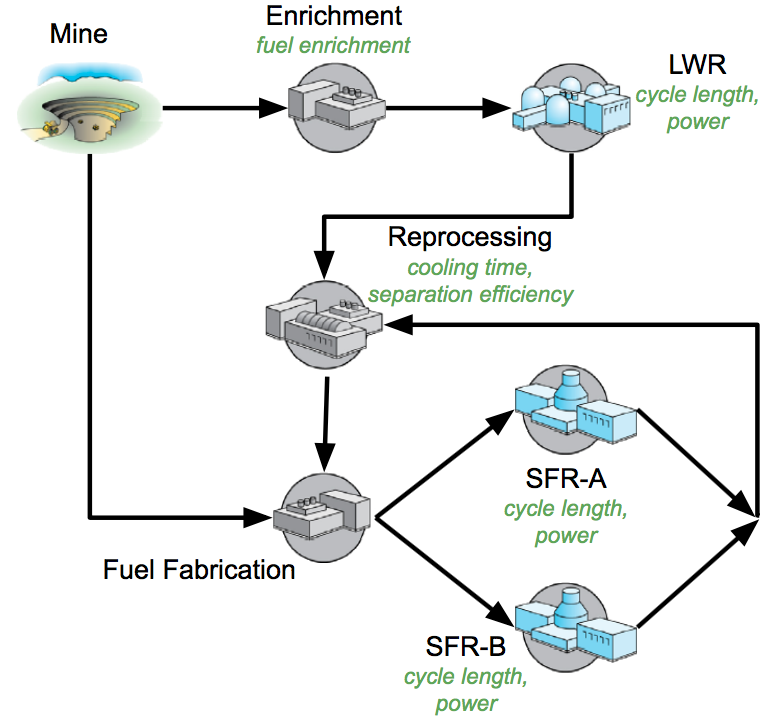
\includegraphics[scale=0.27]{cycle.png}
  \caption{Simplified representation of the material flow between the different facilities,
  with each operational parameter associated with an
  uncertainty labeled in green.}\label{fig:cycle}
\end{figure}


As illustrated in Figure \ref{fig:power}, the transition starts with a fleet
composed of only \glspl{LWR} loaded with enriched \gls{UOX} fuel.  The actual
transition starts around year 35, with the deployment of \glspl{SFR}. The
\glspl{SFR} are loaded with \gls{MOX}, which consists of plutonium blended with
natural uranium.

\begin{figure}[t] % replace 't' with 'b' to force it to be on the bottom
    \centering
    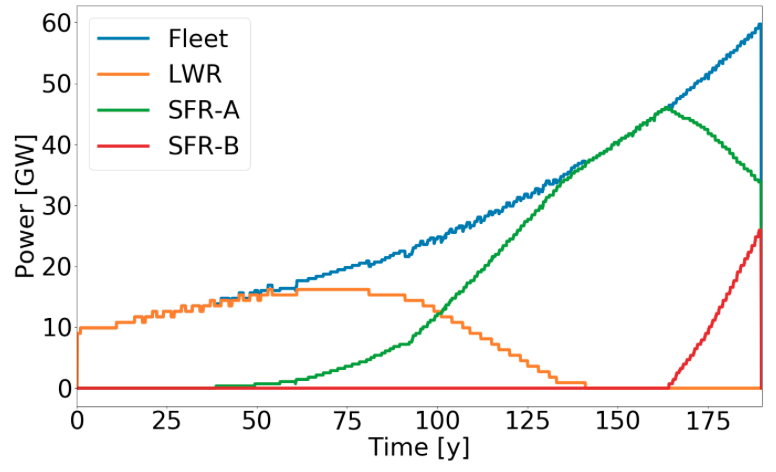
\includegraphics[scale=0.18]{power.png}
    \caption{Electric power generated over time, including contributions from each reactor type.}
    \label{fig:power}
\end{figure}


The plutonium, required for \gls{MOX} fabrication, is reprocessed from all used
fuel.  At first, it is sourced only from \gls{UOX}, then used \gls{MOX} fuel as
it becomes available for reprocessing.

Both fuel reprocessing and fabrication have a constant maximum throughput, but
may also be limited by the availability input material.  The enrichment of the
\gls{UOX} is processed on demand.  Buffer storage facilities (not shown in
Figure \ref{fig:cycle}) are present between all facilities with constant
throughput.

In this work, a time step of 1 month has been considered, \ie each output metric
is reported once per month. Additionally, decay processes have not be taken into
account.  

It must be noted that for this work, the fuel enrichment was determined by a
fuel fabrication model\cite{Leniau2015125} which calculates the fissile fraction
required in the fuel to reach a given target burnup at the end of irradiation.
The target burnup is an operational parameter and does not necessary relate to
the actual achieved burnup (computed from the real cycle length and the thermal
power of the reactor). The uncertainty of the fuel enrichment is not applied
directly to the effective enrichment. It is instead applied to the targeted
burnup, resulting in a fuel enrichment uncertainty that is also close to $10\%$.


A set of 199 simulations was performed in which all five parameters in Table
\ref{tab:package_uncertainty} are randomly varied. Additionally, for each of
those parameters, a set of 199 simulations was performed with only that
parameter being randomly varied, using the \gls{OFAT} method to estimated each
parameter contribution to the overall uncertainty.  A reference simulation was
performed with all five parameters fixed at the mean value.

\section{Results}

Because the main interests of nuclear archaeology involve highly enriched
uranium production and fissile inventories, this study mainly focuses on the
uncertainties of the total quantity of natural uranium used and the total unused
fissile inventory (separated plutonium).

The total power generated in the simulation is reviewed to ensure that none of
the compounded uncertainties result in material shortages substantial enough to
cause long term facility shutdowns.  For example, since \gls{SFR} fuel is built
from reprocessed used fuel, availability of that used fuel may impact the
capability to build the required \gls{SFR}-\gls{MOX} fuel.  While there may be
studies in which this would be an interesting result, in the context of this
work, such shutdowns would be well-documented in the operational histories of
the facilities and should not be characterized as an uncertainty.  Figure
\ref{fig:power_full} shows that uncertainties in generated power are indeed very
low.

\begin{figure}[t] % replace 't' with 'b' to force it to be on the bottom
    \centering
    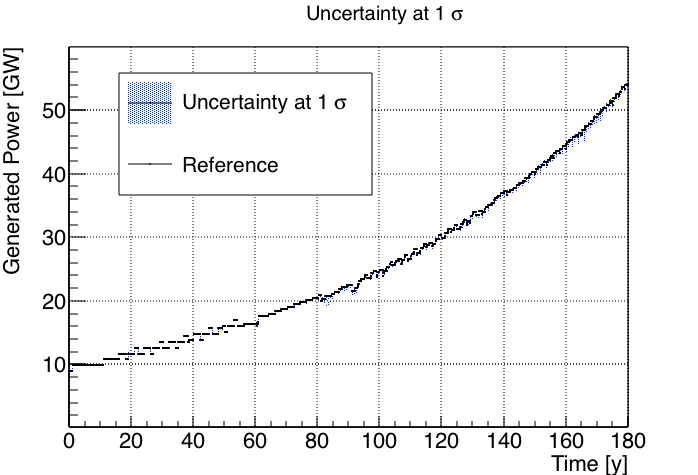
\includegraphics[scale=0.3]{power_full}
    \caption{Electric power generated as a function of time, with its uncertainty.}\label{fig:power_full}
\end{figure}

At each time step, the $\pm1\sigma$ uncertainty due to the full set of varied
parameters is reported.  In addition, the relative contribution to the total
uncertainty from each of the parameters is calculated as the ratio of the
$1\sigma$ uncertainty due to that parameter over the total uncertainty.


\subsection{Natural Uranium Consumption Dedicated to \gls{LWR}-\gls{UOX} fabrication}

Figure \ref{fig:unat_full} represents the cumulative natural uranium consumption
dedicated to \gls{LWR}-\gls{UOX} fuel fabrication as a function of time.  The
uncertainty on the cumulative uranium consumption grows as expected with the
time and the loading of the \glspl{LWR}.  The increase stops around year 125y
with the decommissioning of the last \glspl{LWR}.

As expected, cooling time, separation efficiency and thermal power do not affect
the natural uranium consumption for \gls{LWR}-\gls{UOX} fuel production.  The
uncertainty on the natural uranium consumption is dominated by the \gls{LWR}
cycle length: shorter the cycle length is, the more fuel will be loaded, and
\emph{vice versa}.


\begin{figure}[t] % replace 't' with 'b' to force it to be on the bottom
    \centering
    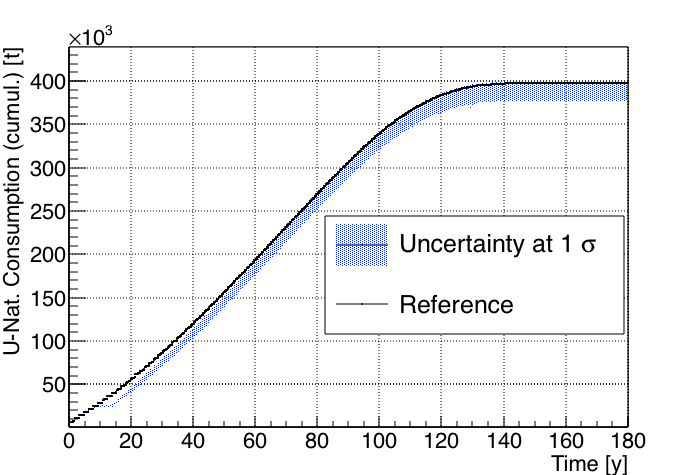
\includegraphics[scale=0.28]{unat_full}
    \caption{Cumulative consumption of natural uranium as a function of time, with
      associated uncertainty.}\label{fig:unat_full}
\end{figure}


\begin{figure}[t] % replace 't' with 'b' to force it to be on the bottom
    \centering
    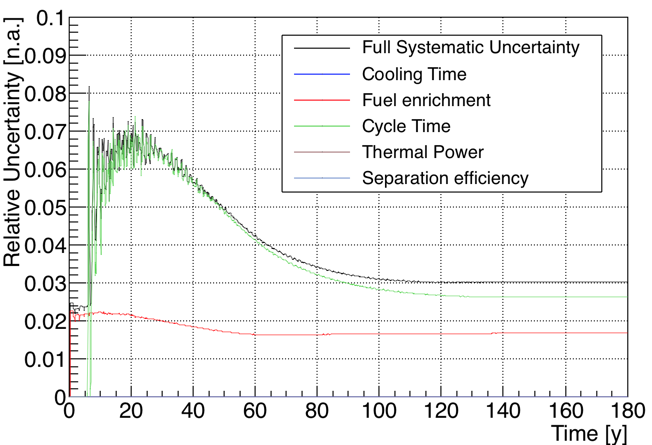
\includegraphics[scale=0.28]{unat_uncer}
    \caption{Relative uncertainty of the cumulative natural uranium consumption, including
      individual contributions from each varied parameter.}\label{fig:unatr_uncer}
\end{figure}

The relative uncertainty of the uranium consumption dedicated to \gls{LWR}
\gls{UOX} fuel fabrication starts at about $7\%$, slowly dropping from year 20
to 100 and stabilizing around $3\%$ after year 100.

Fluctuation of the full relative uncertainty can be observed before year 50.
Those fluctuations are induced by the fuel loading: all reactors at the beginning
of the simulation have synchronized fuel cycles, reloading in the same time
step.  This phenomenon disappears with the gradual decommissioning of the
initial reactors, spread over 50 years.

The decrease of the cycle time uncertainty contribution, from year 30 to year
90, can be understood as an averaging effect.  As the uncertainty are defined
once per deployed facility, each reactor will have a different cycle length
value, so a different number of batches loaded per year.  With the increase of
deployed reactors, the number of batches of \gls{LWR} fuel loaded converges to
the mean (reference) value, reducing its impact on the uncertainty on the
uranium consumption. This uncertainty contribution to the overall uncertainty
decrease is proportional to the number of \gls{LWR} reactors and stops with the
decommission of the last one.

The fuel enrichment contribution follow a close to constant uncertainty
contribution of $2\%$, so as the total relative uncertainty decrease, it
has a growing share of the total absolute uncertainty over time.

\subsection{Fissile Inventory}

The fissile inventory corresponds to the amount of separated fissile material
waiting to be blended with natural uranium in order to produce the
\gls{SFR}-\gls{MOX} fuel.

As observed on Figure \ref{fig:pu_full}, the fissile inventory starts to grow in
year 40, with the deployment of the first reprocessing facility.  It grows
during the first period of the \glspl{LWR} to \gls{SFR}-A transition until year
90, then decrease slightly as the last \glspl{LWR} are decommissioned.  When the
steady state is reached (full \gls{SFR} fleet), the plutonium inventory starts
to increase, as the breading ratio of the \glspl{SFR} is higher than the
deployment needs.

\begin{figure}[t] % replace 't' with 'b' to force it to be on the bottom
    \centering
    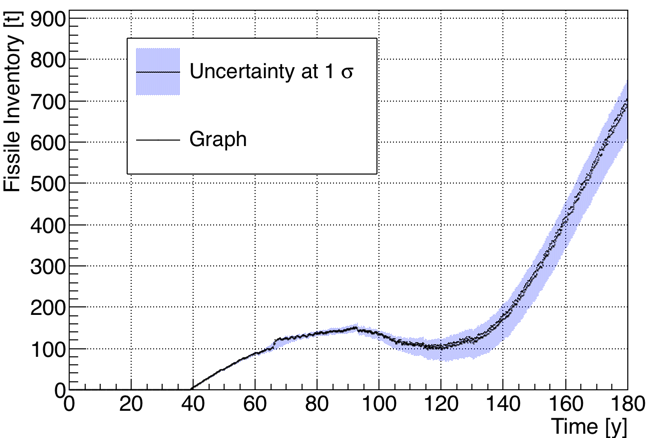
\includegraphics[scale=0.28]{pu_full}
    \caption{Fissile (plutonium) inventory as a function of time, with
      associated uncertainty.}\label{fig:pu_full}
\end{figure}

\begin{figure}[t] % replace 't' with 'b' to force it to be on the bottom
    \centering
    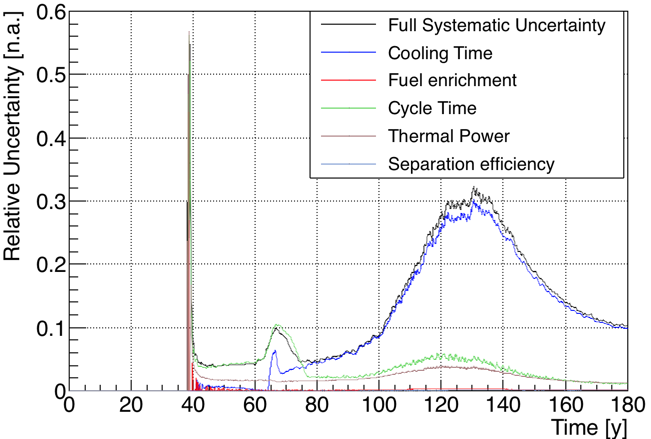
\includegraphics[scale=0.28]{pu_uncer}
    \caption{Relative uncertainty in the fissile (plutonium) inventory, with
      individual contributions from each varied parameter.}\label{fig:pu_uncer}
\end{figure}

At the onset of fissile material production, very low mean inventories lead to
unreliable artifacts in the relative uncertainty.  After that, the relative
uncertainty starts at about $5\%$ and grows until year 125, then decreases to
$10\%$ at the end of the simulation time (180y).  Between year 40 and 70, the
main contributor to the fissile inventory uncertainty is the cycle length.  As
with the uranium needs, different cycle length implies different number of fuel
loads, so different amount of resources used.  Nevertheless, around year 65 (see
Figure \ref{fig:used_fuel}), the stock of used fuel available for reprocessing
becomes small enough to start limiting the production of fissile material.  The
dominant contribution to the uncertainty then slowly transitions from the cycle
length to the fuel cooling time.

\begin{figure}[t] % replace 't' with 'b' to force it to be on the bottom
    \centering
    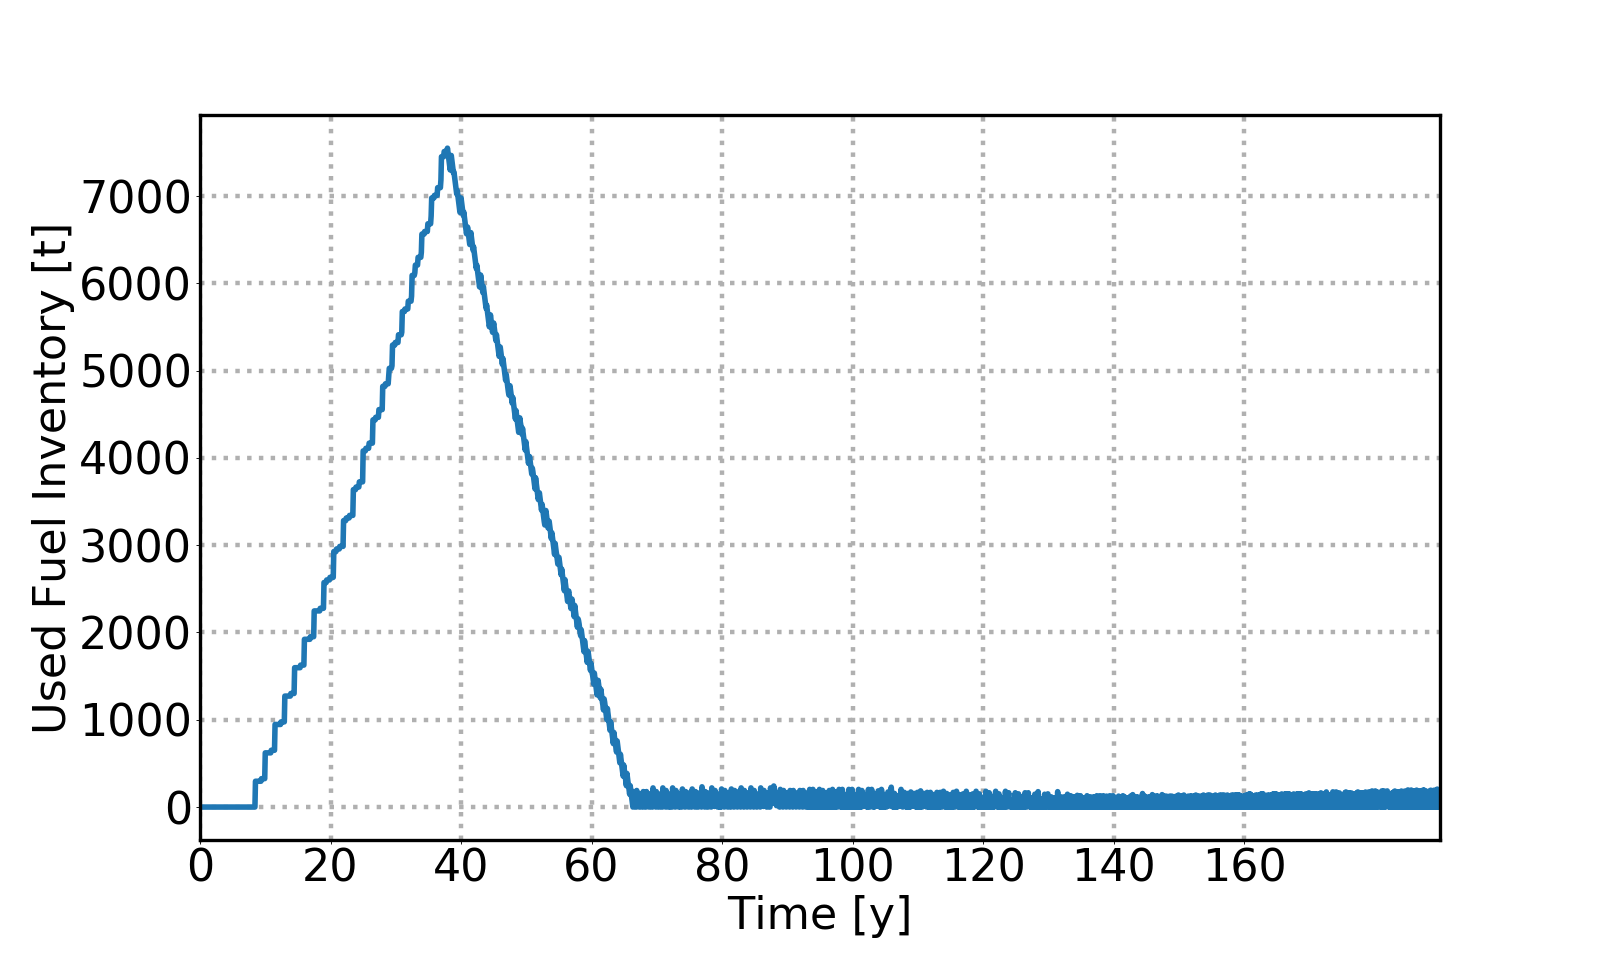
\includegraphics[scale=0.14]{used_fuel}
    \caption{Used fuel inventory, corresponding to the amount of used
    \glspl{LWR} and \glspl{SFR} fuel, cooled and waiting to be reprocessed.}
    \label{fig:used_fuel}
\end{figure}

Between year 90 and 120, the \gls{SFR} deployment speed increases; it has to
compensate the non-replacement of the decommissioned \glspl{LWR} as well as
follow the growing power demand.  During this period the needs in plutonium are
higher than its production, explaining the observed decrease of the total
amount, and the increase associated relative uncertainty.

As the transition ends, the plutonium bred from the \glspl{SFR} starts to be
sufficient to sustain the new \gls{SFR} deployment to follow the power demand.

The uncertainty contribution from the cycle length between year 40 and 70 comes
mainly from fuel batch loading frequencies (Figure \ref{fig:pu_uncer}.  After 70
years this contribution follows the thermal power contribution closely,
suggesting that fuel discharge burnup (\ie fuel discharge composition) is the
mechanism of this contribution, the variation of cycle length driving a
direct variation of the burnup as the thermal power is held constant.  \gls{UOX}
Both the fuel enrichment and separation efficiency showed a relative
contribution smaller than $0.4\%$.

Around the year 70, the relative uncertainty related to cycle time is slightly
bigger than the overall relative uncertainty. This effect is related to the
\gls{OFAT} method used to estimate the individual uncertainty contribution.
While allowing a straightforward estimate of the individual contribution, the \gls{OFAT}
method does not capture coupling effects between the different parameters.

\subsection{Discussion}

Uranium consumption and separated fissile inventory are two important metrics
related to non-proliferation and nuclear archaeology.  In this study, we have
been able to estimate that the cycle length uncertainty of $10\%$ implies a
variation of $3\%$ to $5\%$ on the total uranium needs uncertainty, whereas about
$10\%$ uncertainty on the enrichment implies an almost constant uncertainty of $2\%$.

Regarding the reprocessed fissile inventory, this study has shown the impact of
the reprocessed fuel compositions (through burnup variations) is limited to
$\approx5\%$, while fuel availability constraints, such as fuel loading
frequency (cycle time) or fissile materials available for fuel fabrication
(cooling time) can lead to higher uncertainties, up to $10\%$ and to $30\%$,
respectively.  Moreover, it is very interesting to observe the transition from
one to the other around year 70.

This preliminary study may suggest that the most important contributions to
natural uranium consumption and fissile inventory come from the parameters that
govern the exchange of material between facilities, and not from the physical
parameters that describe those facilities, such as thermal power or fuel
enrichment. Nevertheless such conclusions are specific to this particular scenario
definition: not considering radioactive decay removes the decay of $^{241}$Pu
during cooling, and a transition to fast reactors minimizes the
impact of the change in discharge composition induced by the cycle length
variations when reprocessing spent fuel to build the next \gls{MOX} fuel batch.

\section{Conclusion}

Three main points can be deduced from this work.  First, in a transitional fuel
cycle, uncertainty contributions to output metrics can vary over time depending
of various factors: deployment schedule artifacts or material flow
constrictions.

Second, it is important to note the special character of the time related
parameters uncertainty in a fuel cycle study, such as cooling time and cycle
length.  While some of those time related parameters will, to first order, only
impact material availability (as the cooling time will do), others, like cycle
length, will also have a impact as physical parameters such as fuel enrichment
or thermal power.  

Finally, Figure \ref{fig:pu_uncer} shows the limit of the \gls{OFAT} method to
assess the individual contribution of each parameter, missing all the coupling
effects between them. 

Cycle length impacts the discharge fuel burnup and the frequency of the fuel
loads.  When they combine to produce in uncertainty of the material
availability, this could result in variations related to time delays that may
contribute to the final uncertainty in ways that are not relevant to some
analyses.  That is, a simple time lag in a particular output that otherwise
follows an identical history could manifest itself as a large variation at any
particular time.  Those kind of time related uncertainties will require a
further analysis to understand and measure accurately their contributions to the
total uncertainty. 

This study aims to be a proof-of-principle for uncertainty propagation in
potential commercial fuel cycle transition.  While it has demonstrated the
capability to measure the uncertainty on output fuel cycle metrics and their
relative contributions, it has only been applied to systematic uncertainties per
facilities.  This kind of study will be extended to random uncertainty (new
parameter values as a function of time) and completely systematic uncertainty
(shared by all the facilities of a kind). Additionally more sophisticated
methods needs to be used to assess precisely each parameter contributions..

Such studies could provide research guidance for nuclear archaeology work,
which aims to precisely estimate past fissile production by the different
nuclear countries.




%%%%%%%%%%%%%%%%%%%%%%%%%%%%%%%%%%%%%%%%%%%%%%%%%%%%%%%%%%%%%%%%%%%%%%%%%%%%%%%%
\section{Acknowledgments}
This work was funded by the Consortium for Verification Technology under
Department of Energy National Nuclear Security Administration award number
DE-NA0002534

%%%%%%%%%%%%%%%%%%%%%%%%%%%%%%%%%%%%%%%%%%%%%%%%%%%%%%%%%%%%%%%%%%%%%%%%%%%%%%%%
\bibliographystyle{ans}
\bibliography{bibliography}
\end{document}
